
\section{Graph Creation}

\subsection{Node Pruning}

We remove all nodes from the graph corresponding to labels with fewer than $t_{seg}$ voxels (Section 3.1).
Figure \ref{fig:node-pruning} shows the results of varying $t_{seg}$ on two different quantities for the Kasthuri training volume. 
The blue line indicates the number of nodes remaining in the graph.
The rate of node reduction decreases for larger thresholds since there are fewer labels of larger size. 
The green line shows the percent of voxels with a label pruned from the graph.
Ideally this number is low since we want to remove small segments which do not contribute much to the overall volume.
These are locations which we cannot improve the variation of information scores.
This ``volume lost" grows at an increasing rate as the larger segments are removed. 
Based on these curves we set $t_{seg} = 20000$ voxels.
With this threshold, we prune over half of the labels that correspond to around $1.5\%$ of the total volume.

\subsection{Edge Pruning}

There are two parameters in the two-pass edge pruning algorithm, $t_{low}$ and $t_{high}$ (Section 3.2). 
The resulting graph should have the highest possible percentage of split errors still present while keeping the number of total edges low. 
We perform a search over varying thresholds for $40\textrm{nm} \leq t_{low} \leq 300 \textrm{nm}$ and $300 \textrm{nm} \leq t_{high} \leq 800 \textrm{nm}$ on the Kasthuri training dataset to find the parameter with the highest retention of true splits that keeps the number of total edges less than $6 \times$ the number of split errors. 

\begin{figure}
	\begin{center}
		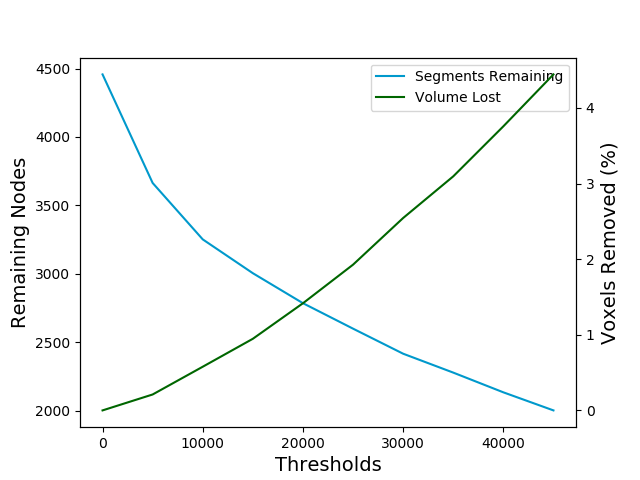
\includegraphics[width=0.95\linewidth]{./figures/node-threshold.png}
		\caption{The number of remaining nodes after increasing the threshold (blue) and the number of voxels with this label as a percent of the total volume (green). }
		\label{fig:node-pruning}
	\end{center}
\end{figure}
